\section{Introduction}
% VizWiz, es el proyecto responsable de introducir los primeros conjuntos de datos y retos, destinados a motivar la creación de nuevas y mejores tecnología/algoritmos asistenciales de inteligencia artificial, para ayudar a personas con discapacidades visuales.
% En 2010, Bigham et al. [6] presenta VizWiz, una aplicación de teléfono móvil destinada a ayudar a personas no videntes en sus problemas diarios. Los usuarios tomaban una fotografía y grababan una pregunta sobre lo que querían conocer de esa imagen. Tales preguntas visuales, eran respondidas por un grupo de trabajadores, mayoritariamente reclutados de empresas como Amazon Mechanical Turk.
% Ocho años después, Gurari et al. [3] filtraron y anonimizaron la información de todos los datos recopilados hasta ese momento, y para cada par de imágenes y preguntas, recolectaron un total de 10 respuestas provenientes de fuentes múltiples. Esto, llevo a que en la conferencia de Computer Vision and Patter Recognition 2018 (CVPR 18) se presentara el primer conjunto de datos VQA público `orientado a objetivos' no artificial, construido totalmente de datos originados por  personas no videntes. La Figura (\ref{fig:vizwiz_samples}) ilustra algunos ejemplos de esta dataset.
VizWiz\footnote {\url{https://vizwiz.org}}, is the project responsible for introducing the first datasets and challenges, aimed at motivating the creation of new and better AI assistive technology/algorithms, to help people with visual impairment.
In 2010, Bigham et al. \cite{vizwiz_phone} presents VizWiz, a mobile phone application designed to help blind people with their daily problems. Users took a photo and recorded a question about what they wanted to know about that image. Such visual questions were answered by a group of workers, mostly recruited from companies like Amazon Mechanical Turk.
Eight years later, Gurari et al. \cite{vizwiz_grandchallenge} filtered and anonymized the information from all the data collected up to that point, and for each pair of images/questions, they collected a total of 10 answers using crowd-sources. In the Computer Vision and Pattern Recognition 2018 conference (CVPR 18), they presenting the first non-artificial 'goal-oriented' public VQA data-set, built entirely from data originated by blind people. Figure (\ref{fig:vizwiz_samples}) illustrates some examples of this dataset.

\begin{figure}[ht!]
    \centering
    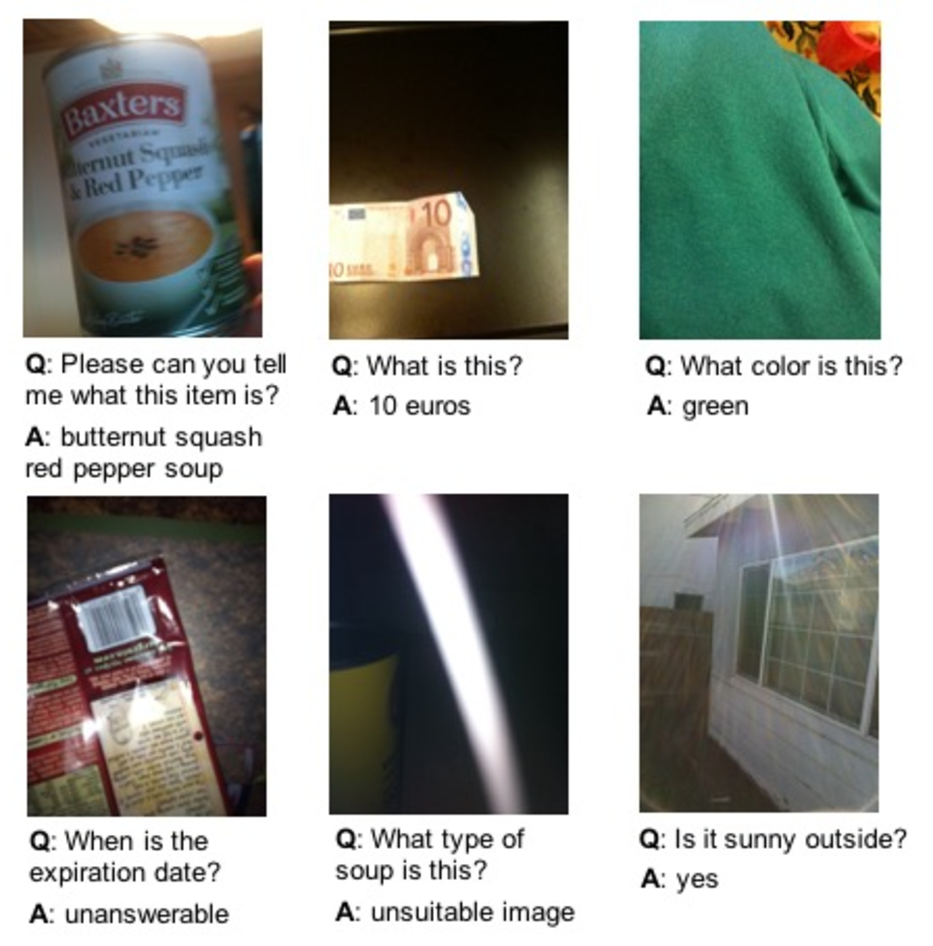
\includegraphics[width=\linewidth]{images/intro/vizwiz_samples.pdf}
\caption{Samples of VizWiz-VQA dataset.}
\label{fig:vizwiz_samples}
\end{figure}


\paragraph{\textbf{VizWiz-VQA.}}
% Dado a que las mismas personas no videntes fueron las responsables de capturar las fotografías y grabar las preguntas, gran parte de las imágenes de este conjunto de datos, se caracterizan por presentar problemas de enfoque, iluminación y encuadre. Por otro lado, las preguntas son marcadamente conversacionales, ya que no se hablan como se escribe, y gran parte de ellas aparecen incompletas como consecuencias de cortes e imperfecciones en los audios de las que fueron transcritas.
% Como resultado, ya sea porque la pregunta no pudo ser respondida del contexto de la imagen, o porque la calidad de la imagen era inadecuada, VizWiz-VQA cuenta con una gran cantidad de preguntas visuales que no pueden ser respondidas, diferenciándolo del resto de datasets VQA.
Since the same blind people were responsible for capturing the photographs and recording the questions, a large part of the images in this data set are characterized by focusing, lighting and framing problems. On the other hand, since people speak differently from how they write, the data set is markedly conversational. With a large majority of incomplete questions due to cuts and imperfections in the audios from which they were transcribed.
As a result, either because the question could not be answered from the context of the image, or because the image quality was unsuitable, VizWiz-VQA has a large number of visual questions that cannot be answered, unlike other VQA datasets.

% Específicamente, el conjunto esta formado por 20523 pares image/question y 205230 respuesta asociadas para el grupo de entrenamiento; 4319 pares de image/question y 43190 respuestas asociadas para el grupo de validación; y 8000 pares de image/question en el grupo de testeo. Cada una de las preguntas poseen asignada una categoría, la cual hereda del tipo de respuesta esperada (los valores entre paréntesis representan la frecuencia en el dataset): `number' ($\sim$1,4\%), `yes/no' ($\sim$4,63\%), `unanswerable' ($\sim$27,84\%) y `other' ($\sim$66,1\%).
% La longitud media de cada pregunta ronda las $\sim$6.8 palabras, y aproximadamente el 28\% de las palabras iniciales aparecen menos del 5\% de la veces en el conjunto. Esto último, atribuido a la naturaleza conversacional del conjunto, donde preguntas del estilo “Hi, can you please tell me which is . . . ” in VizWiz, se encuentra simplemente como “Which is . . . ” en conjunts como VQA v2.0.

Specifically, VizWIz-VQA\footnote {\url{https://vizwiz.org/tasks-and-datasets/vqa/}} is conformed of 20523 images/questions pairs, and 205230 associated answers in the training set; 4319 image/question pairs, and 43190 associated answers in the validation set; and 8000 pairs of images/questions in the test set. Each of the questions is assigned a category, which inherits the type of expected answer (the values in parentheses represent the frequency in the dataset): `number' ($\sim$1,4\%), `yes/no' ($\sim$4.63\%), `unanswerable' ($\sim$27.84\%) and `other' ($\sim$66.1\%).
The average length of each question is around $\sim$6.8 words, and approximately 28\% of the opening words appear less than 5\% of the time in the set. The latter, attributed to the conversational nature of the set, where questions such as ``Hi, can you please tell me which is . . . '' in VizWiz, it is found simply as ``Which is. . . '' in datasets like VQA v2.0\footnote{\url{https://visualqa.org/}}.

\paragraph{\textbf{Contributions.}}
% En este trabajo, como consecuencia del análisis de  $\sim$24800 pares de preguntas y respuestas provenientes de los conjuntos de entrenamiento y validación, se realizaron las siguientes contribuciones:
% \begin{itemize}
%     \item Exploración e identificación de estrategias de pre-procesamiento y clusterización, para la desagregación consistente de grupos de preguntas mayoritarias del conjunto VizWiz-VQA.
%     \item Definición de ocho nuevas categorías, para identificar y caracterizar de una manera más descriptiva y natural, al conjunto total de preguntas de VizWiz-VQA.
%     \item Entrenamiento y testeo de modelo de clasificación automática sobre las nuevas categorías definidas, y análisis de las categorías originaes `other' y `unanswerable' en base a nuevas clasificaciones obtenidas.
% \end{itemize}
In this work, as a consequence of the analysis of $\sim$24.800 pairs of questions and answers from the training and validation sets, the following contributions were made:
\begin{itemize}
    \item Exploration and identification of pre-processing and clustering strategies, for the consistent disaggregation of groups of majority questions of the VizWiz-VQA dataset.
    \item Definition of eight new main categories, to identify and characterize in a more descriptive and natural way, the total set of VizWiz-VQA questions.
    \item Training and testing of the automatic classification model on the new defined categories, and analysis of the original categories, mainly the `other' and `unanswerable'  clases, based on the new classifications obtained.
\end{itemize}